%\begin{Exercise}[label=Ex2]
\Exercise[title=Substitució]
$\int \frac{1}{x^2 \sqrt{4-x^2}}dx$ (pista: usa dues substitucions consecutives)

%\end{Exercise}

%\begin{Answer}[ref=Ex2]
\Answer
Ens hem d'adonar que tenim una arrel de la forma $\sqrt{a^2-x^2}$. En aquests casos podem mirar de transformar l'arrel en quelcom del tipus $\sqrt{1-\sin^2{x}}$. Per tant, comencem plantejant el canvi
\[
  x=2\cos{t}; \; dx=-2\sin{t}dt
\]
I per tant:
\begin{eqnarray*}
  \int \frac{1}{x^2 \sqrt{4-x^2}}dx
  &=& \int \frac{-2\sin{t}}{4\cos^2{t}\sqrt{4-4\cos^2{t}}} dt = \int \frac{-2\sin{t}}{8\cos^2{t}\sqrt{1-\cos^2{t}}} dt\\
  &=& \int \frac{-2\sin{t}}{8\cos^2{t}\sqrt{\sin^2{t}}} dt = -\frac{1}{4} \int \frac{dt}{\cos^2{t}} dt=-\frac{1}{4} \tan{t}
\end{eqnarray*}

Ara podem desfer el canvi de variable fent $x=2\cos{t} \Rightarrow t=\arccos{\frac{x}{2}}$

\[
  \int \frac{1}{x^2 \sqrt{4-x^2}}dx=-\frac{1}{4} \tan{\arccos{\frac{x}{2}}}
\]

Ho podem deixar així o podem pensar en que si $\alpha=\arccos{\frac{x}{2}}$, segons el dibuix  $\tan{\arccos{\frac{x}{2}}}=\tan{\alpha}=\frac{\sqrt{1-\frac{x}{2}}}{\frac{x}{2}}$.

\begin{center}
  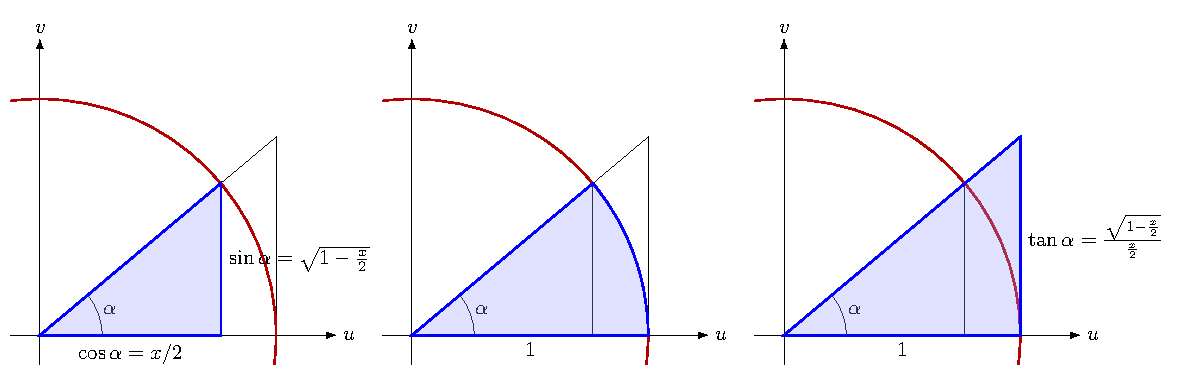
\includegraphics[width=0.8\textwidth]{Ex2unitcircle.pdf}
\end{center}

Per tant, per a $x=2\cos{t}$: 

\[
\int \frac{1}{x^2 \sqrt{4-x^2}}dx = -\frac{1}{4} \tan{t} = -\frac{1}{4}\frac{\sqrt{1-\frac{x}{2}}}{\frac{x}{2}}
\]

%\end{Answer}
